%
% euler.tex
%
% (c) 2020 Prof Dr Andreas Müller, Hochschule Rapperswil
%
\begin{frame}[fragile]
\frametitle{Euler-Verfahren}
\vspace{-15pt}
\begin{columns}[t]
\begin{column}{0.48\hsize}
\begin{center}
\begin{tikzpicture}[>=latex,thick]

\def\exaktekurve#1{
	\draw[color=red]
		plot[domain=-0.2:5,samples=100] ({\x},{1+\x+(#1-1)*exp(\x)});
}

\def\kurve#1{
	\pgfmathparse{5/#1}
	\xdef\h{\pgfmathresult}
	\node[color=blue] at (3.2,4.0) [right] {$h=\h$};
	\xdef\x{0}
	\xdef\y{0.95}
	\foreach \k in {1,...,#1}{
		\pgfmathparse{\y-\x}
		\xdef\yprime{\pgfmathresult}
		\fill[color=blue] ({\x},{\y}) circle[radius=0.04];
		\draw[color=blue] ({\x},{\y})--({\x+\h},{\y+(\h*\yprime)});
		\pgfmathparse{\y+\h*\yprime}
		\xdef\y{\pgfmathresult}
		\pgfmathparse{\x+\h}
		\xdef\x{\pgfmathresult}
	}
	\fill[color=blue] ({\x},{\y}) circle[radius=0.04];
}


\uncover<3->{
\begin{scope}
\clip (-0.1,-0.1) rectangle (5,5.6);
\foreach \yzero in {0,0.1,...,2}{
	\exaktekurve{\yzero}
}
\exaktekurve{0.95}
\end{scope}
}

\fill[color=blue] (0,0.95) circle[radius=0.06];

\begin{scope}
\clip (-0.1,-0.1) rectangle (5.3,5.7);
\only<6>{ \kurve{10} }
\only<7>{ \kurve{20} }
\only<8>{ \kurve{40} }
\only<9>{ \kurve{80} }
\only<10>{ \kurve{160} }
\end{scope}

\draw[->] (-0.1,0)--(5.8,0) coordinate[label={$x$}];
\draw[->] (0,-0.1)--(0,5.8) coordinate[label={right:$y$}];
\end{tikzpicture}
\end{center}
\end{column}
\begin{column}{0.48\hsize}
\begin{block}{Aufgabe}
\vspace{-20pt}
\begin{align*}
y'&=y - x\\
y(0)&=0.95
\end{align*}
\end{block}
\vspace{-15pt}
\uncover<2->{%
\begin{block}{Analytische Lösung}
\vspace{-18pt}
\begin{align*}
y(x)
&=
\underbrace{1+x}_{\displaystyle=y_p(x)}
+
(0.95-1)\underbrace{e^{x}}_{\displaystyle=y_h(x)}
\end{align*}
\end{block}}
\vspace{-18pt}
\uncover<4->{%
\begin{block}{Iterativ nach Euler}
\vspace{-18pt}
\begin{align*}
y(h)&= y(0) + y'(0)\cdot h = 0.95 + 0.95\cdot h
\\
\uncover<5->{y(kh)}&\uncover<5->{=y((k-1)h) + y'((k-1)h)\cdot h}
\end{align*}
\end{block}}
\end{column}
\end{columns}
\end{frame}
